\documentclass{curs}

% Comment out lines below in case of no code to be included.
%\usepackage{code/highlight}
\usepackage{color}
\usepackage{graphicx}
%\usepackage{alltt}


\title[Session 02]{Session 02}
\subtitle{Authentication}
\author{Security of Information Systems (SIS)}
\date{October 13, 2017}

\begin{document}

\frame{\titlepage}


\section{Authentication}

\begin{frame}{Model}
  \begin{itemize}
    \item Actor
    \item Role
    \item Database
  \end{itemize}
\end{frame}

\begin{frame}{Credentials}
  \begin{itemize}
    \item Who you are
    \item What you have
    \item What you know
  \end{itemize}
\end{frame}

\begin{frame}{Credential types}
  \begin{itemize}
    \item Biometric
    \item Hardware tokens
    \item Software tokens
    \item Secret (Password)
  \end{itemize}
\end{frame}


\section{Credentials}

\begin{frame}{Biometrics}
  \begin{itemize}
    \item Fingerprint
    \item Face
    \item Iris
    \item Voice
    \item Keystroke dynamics
  \end{itemize}
\end{frame}

\begin{frame}{Hardware tokens}
  \begin{itemize}
      \item Access card
      \item Hardware keys
      \item OneTimePassword
    \end{itemize}
\end{frame}

\begin{frame}{Software tokens}
  \begin{itemize}
    \item Certificate
    \item Kerberos ticket
    \item Cookie
  \end{itemize}
\end{frame}

\section {Passwords}

\begin{frame}{Passwords}
  \begin{itemize}
    \item string of printable characters (ASCII)
    \item protect access
    \item stored in a password database and requested at each
      login/authentication
    \item most common method of authentication
  \end{itemize}
\end{frame}

\begin{frame}{Password Cracking Context (1)}
  \begin{figure}
    \centering
    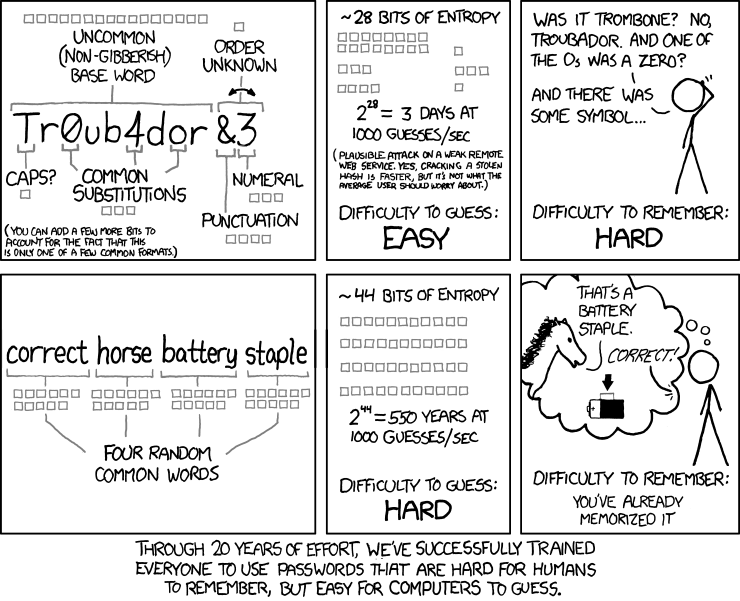
\includegraphics[width=0.8\textwidth]{img/password-strength.png} \\
    \tiny{\url{http://xkcd.com/936/}}
  \end{figure}
\end{frame}

\begin{frame}{Password Cracking Context (2)}
  \begin{figure}
    \centering
    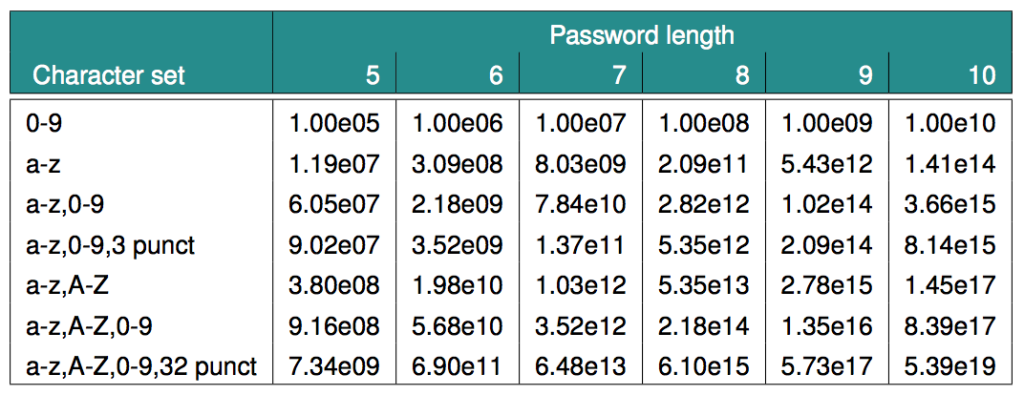
\includegraphics[width=0.8\textwidth]{img/password-complexity.png} \\
    \tiny{\url{http://hitachi-id.com/password-manager/docs/password-management-best-practices.pdf}}
  \end{figure}
\end{frame}

\begin{frame}{Passwords vs. Passphrases}
  \begin{itemize}
    \item A password is a word and a passphrase is a set of words
    \item Passphrases usually has spaces
    \item Passphrases are recommended due to their increased length and being
      easier to remember
  \end{itemize}
\end{frame}

\begin{frame}{Attacker}
  \begin{itemize}
    \item Online attack
      \begin{itemize}
        \item ``live'' attack
        \item run client/application, feed passwords and try to match
      \end{itemize}
    \item Offline attack
  \end{itemize}
\end{frame}

\section {Scenario 1}

\begin{frame}{Scenario 1: Plaintext}
  \begin{itemize}
    \item Attacker \begin{itemize}
      \item Gain access to database
      \item Profit!
    \end{itemize}
    \item Defender \begin{itemize}
      \item Database ACL
      \item One way function
    \end{itemize}
  \end{itemize}
\end{frame}

\begin{frame}{Cryptographic hash function}
  \begin{itemize}
    \item Deterministic
    \item Uniformity
    \item Infeasible to reverse
    \item Highly dynamic
    \item Usually very fast
  \end{itemize}
\end{frame}

\begin{frame}{Hash security properties}
  \begin{itemize}
    \item Pre-image resistance
    \item Second pre-image resistance
    \item Collision resistance
  \end{itemize}
\end{frame}

\begin{frame}{Hash algorithms}
  \begin{itemize}
    \item \color{red}SHA1
    \item \color{red}MD2, MD4, MD5
    \item \color{lime}SHA2
    \item \color{green}bcrypt
    \item \color{green}SHA3
  \end{itemize}
\end{frame}

\section {Scenario 2}

\begin{frame}{Scenario 2: Hashed password}
  \begin{itemize}
    \item Attacker \begin{itemize}
      \item Rainbow tables
      \item Profit!
    \end{itemize}
    \item Defender \begin{itemize}
      \item Salt
    \end{itemize}
  \end{itemize}
\end{frame}


\begin{frame}{Rainbow Tables}
  \begin{itemize}
    \item Database of hashes
    \item Space vs time
  \end{itemize}
\end{frame}

\begin{frame}{Rainbow Tables (2)}
  \begin{figure}
    \centering
    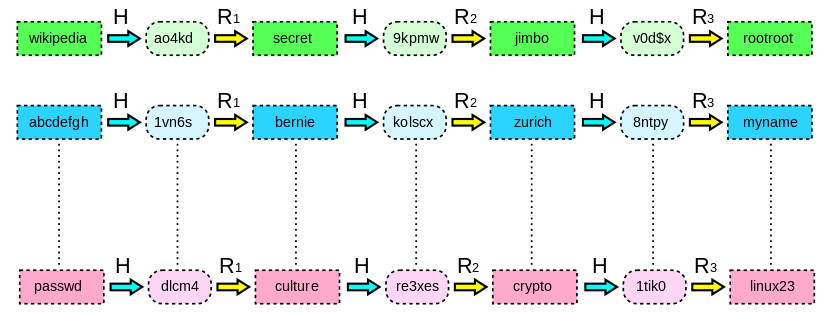
\includegraphics[width=0.9\textwidth]{img/rainbow-table.png} \\
    \tiny{\url{http://en.wikipedia.org/wiki/Rainbow_table}}
  \end{figure}
\end{frame}

\begin{frame}{Salt}
  \begin{itemize}
    \item Additional input
    \item Concatenated with the password
    \item One per password
  \end{itemize}
\end{frame}

\section {Scenario 3}

\begin{frame}{Scenario 3: Salted hashes}
  \begin{itemize}
    \item Attacker
      \begin{itemize}
        \item Dictionary/hybrid attack
        \item Brute force attack
        \item Side channel attacks
        \item Profit ?!?
      \end{itemize}
    \item Defender \begin{itemize}
      \item Policies
      \item Defensive programming
    \end{itemize}
  \end{itemize}
\end{frame}

\begin{frame}{Dictionary Attacks}
  \begin{itemize}
    \item use a dictionary/word list
    \item go through word list, compute hash and compare to password hash
    \item simple form of attack
    \item relies on people using simple passwords
  \end{itemize}
\end{frame}

\begin{frame}{Password Dictionaries/Word Lists}
  \begin{itemize}
    \item \url{http://wiki.skullsecurity.org/Passwords}
    \item
      \url{https://crackstation.net/buy-crackstation-wordlist-password-cracking-dictionary.htm}
    \item
      \url{http://security.stackexchange.com/questions/9567/modern-high-quality-password-dictionary}
  \end{itemize}
\end{frame}

\begin{frame}{Hybrid attack}
  \begin{itemize}
    \item Use a dictionary
    \item Apply mutations for each word
      \begin{itemize}
       \item combine dictionary words
        \item change i to 1, s to 5, e to 3
        \item change cases
        \item add 123 at the end of the word
        \item add ! at the end of the word
      \end{itemize}
    \item Hash and check with password hash
  \end{itemize}
\end{frame}

\begin{frame}{Policy}
  \begin{itemize}
    \item Complexity
      \begin{itemize}
        \item Password length
        \item Charset
      \end{itemize}
    \item Password expiration
    \item Password reuse
  \end{itemize}
\end{frame}

\begin{frame}{Policy issues}
  \begin{itemize}
    \item Password security paradox
      \begin{itemize}
        \item Easy to remember
        \item Hard to guess
      \end{itemize}
    \item User behavior
    \item Solution: Password managers
  \end{itemize}
\end{frame}

\begin{frame}{Side channel attacks}
  \begin{itemize}
    \item Timing information
    \item Performance / power consumption 
    \item Electromagnetic leak
    \item Acoustic information
    \item Social engineering
    \item Rubber-hose technique
  \end{itemize}
\end{frame}

\begin{frame}{Rubber-hose technique}
  \begin{figure}
    \centering
    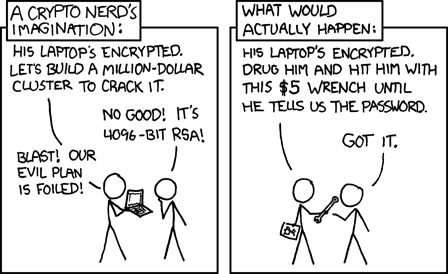
\includegraphics[width=0.8\textwidth]{img/security-wrench.png} \\
    \tiny{\url{http://xkcd.com/538/}}
  \end{figure}
\end{frame}


\section{Summary}

\begin{frame}{Recommendations}
  \begin{itemize}
    \item Do not use unsafe hashing algorithms!!!
    \item Passphrase $>$ complex password
    \item Use/allow password managers
    \item Use 2FA/3FA
    \item Secure side channels
  \end{itemize}
\end{frame}

\begin{frame}{Common tools}
  \begin{itemize}
    \item \href{http://www.openwall.com/john/}{John The Ripper}
    \item \href{http://project-rainbowcrack.com/}{RainbowCrack}
    \item \href{https://hashcat.net/hashcat/}{HashCat}
  \end{itemize}
\end{frame}

\begin{frame}{Keywords}
  \begin{columns}
    \begin{column}{0.5\textwidth}
      \begin{itemize}
        \item Credentials
        \item Password
        \item Passphrase
        \item Hash functions
        \item Rainbow tables
        \item Salt
        \item Dictionary attack
        \item Side channel attack
        \item Policies
      \end{itemize}
    \end{column}
    \begin{column}{0.5\textwidth}
      \begin{itemize}
        \item Social engineering
        \item Shoulder surfing
        \item One time password
        \item Password complexity
        \item Password manager
        \item 2/3 Factor authentication
        \item SHA256,SHA512
        \item SHA3
        \item Rubber hose technique
      \end{itemize}
    \end{column}
  \end{columns}
\end{frame}

\begin{frame}{Nice to read}
  \begin{itemize}
    \item \href{http://books.expect-us.net/dl/Password_Cracking_Techniques.pdf}{Password Cracking Techniques}
    \item \href{https://arstechnica.com/information-technology/2017/05/breaking-the-iris-scanner-locking-samsungs-galaxy-s8-is-laughably-easy/}{Breaking the iris scanner locking Samsung’s Galaxy S8 is laughably easy}
    \item \href{https://arstechnica.com/gadgets/2017/03/video-shows-galaxy-s8-face-recognition-can-be-defeated-with-a-picture/}{Galaxy S8 face recognition already defeated with a simple picture}
    \item \href{https://arstechnica.com/information-technology/2013/09/touchid-hack-was-no-challenge-at-all-hacker-tells-ars/}{Bypassing TouchID was “no challenge at all,” hacker tells Ars}
    \item \href{https://paul.reviews/behavioral-profiling-the-password-you-cant-change/}{Behavioral Profiling: The password you can't change.}
  \end{itemize}
\end{frame}
\end{document}
